\documentclass[10pt,twocolumn]{article}
\usepackage[margin=0.62in,columnsep=0.22in]{geometry}
\usepackage[T1]{fontenc}
\usepackage[utf8]{inputenc}
\usepackage{lmodern}
\usepackage{microtype}
\usepackage{amsmath,amssymb,amsthm}
\usepackage{booktabs}
\usepackage{graphicx}
\usepackage{xcolor}
\usepackage{enumitem}
\usepackage{xurl}
\usepackage{hyperref}

\hypersetup{
  colorlinks=true,
  linkcolor=blue!60!black,
  citecolor=blue!60!black,
  urlcolor=blue!60!black,
  pdftitle={Constructive Lean 4 Kernel and Exact Zero-Float Certificates for OpenAI Matching Matrix Multiplication Lower Bound 9/4},
  pdfauthor={Lluis Eriksson}
}

\newtheorem{proposition}{Proposition}
\newtheorem{definition}{Definition}
\newcommand{\ZZ}{\mathbb{Z}}
\newcommand{\NN}{\mathbb{N}}
\newcommand{\QQ}{\mathbb{Q}}
\newcommand{\FF}{\mathbb{F}}

\title{\vspace{-0.9em}\textbf{Constructive Lean~4 Kernel and Exact Zero-Float Certificates for OpenAI's Matching Matrix Multiplication Lower Bound $\omega_F = 9/4$}}
\author{Lluis Eriksson\thanks{Independent Researcher. Code, Lean~4 proofs, and certificates: MIT License; manuscript and figures: CC-BY-4.0. Prepared with transparent AI coding, formalization, and drafting assistance via Google Antigravity; all Lean~4 theorems, exact zero-float verifiers, and adversarial tests were independently compiled and verified locally. Repository: \href{https://github.com/lluiseriksson/openai-omega-nine-fourths-lower-bound-certificates}{\nolinkurl{github.com/lluiseriksson/openai-omega-nine-fourths-lower-bound-certificates}}.}}
\date{November 25, 2026}

\begin{document}
\maketitle
\vspace{-1.2em}

\begin{abstract}
A November~24, 2026 companion preprint from OpenAI~\cite{openai2026omega94} proposes a matching lower bound showing that the exponent of square matrix multiplication equals $\omega_F = 9/4$ over every field $F$, with geometric border rank $\underline{R}(T_n)\ge n^{9/4}$, at least $\lceil n^{9/4}/2\rceil$ nonscalar multiplication or division gates for every $n\ge 2$, dual exponent $\alpha_F\le 2/3$, and a refutation of Strassen's tight-tensor conjecture. Rather than assuming peer-reviewed endorsement of its $\mathrm{CAT}(0)$ spectral-space and tensor-network compression pillars, we deliver an independent, explicitly scoped, zero-floating-point verification companion for its discrete algebraic, symbolic dual-number bilinearization, tight-support, tagged-permutation, harmonic-star, and tripod arithmetic--harmonic mean (AM--HM) rigidity mechanisms. Layer~1 (\nolinkurl{OpenAIOmegaLowerBound.lean}) proves 18 standalone constructive Lean~4.35.0 algebraic, combinatorial, and rational-rigidity sub-lemmas (zero \texttt{sorry}, zero \texttt{axiom}, zero \texttt{Classical.choice}, zero warnings; 4 zero-axiom \texttt{none} and 14 \texttt{[propext, Quot.sound]}). Layer~2 (\texttt{OMEGA94-\allowbreak LB-\allowbreak CERT-1.0}) is a pure-stdlib Python \texttt{int}/\texttt{Fraction} 4-mode auditor certifying 16 canonical finite witnesses in $0.027$--$2.466\,\mathrm{ms}$ and rejecting 70/70 live adversarial forgeries with exact branch assertions (76/76 pytest checks).
\end{abstract}

\section{Introduction and Scope Calibration}\label{sec:intro}
Since Strassen's seven-product algorithm~\cite{strassen1969gaussian}, the matrix multiplication exponent $\omega_F$ has been a central open problem in algebraic complexity. On the lower-bound side, Bl\"aser proved ordinary rank $\ge \frac{5}{2}n^2-3n$~\cite{blaser2000lower} and Landsberg--Micha{\l}ek proved border rank $\ge 2n^2-\lceil\log_2 n\rceil-1$~\cite{landsberg2018lower}, leaving the asymptotic exponent lower bound stuck at $2$. Following the $9/4$ upper bound established over $\mathbb{C}$ by OpenAI~\cite{openai2026omegaupper} and over every field $F$ by Amanov, van den Berg, and Zuiddam~\cite{amanov2026omega}, OpenAI's November~24, 2026 companion preprint~\cite{openai2026omega94} proposes the matching lower bound $\omega_F = 9/4$ over every field $F$ via four discrete-algebraic and geometric pillars:
\begin{enumerate}[leftmargin=1.2em,itemsep=1pt,topsep=2pt]
  \item \textbf{Finite-Size Rank, Gate, Rectangular \& Tight-Tensor Consequences (Cors.~1.2--1.3, Sec.~2.4):} $\underline{R}(T_n)\ge n^{9/4}$ yields $\ge\lceil n^{9/4}/2\rceil$ nonscalar gates, rectangular bound $\underline{R}(T_{a,b,c})\ge\max\{ab,bc,ca,(abc)^{3/4}\}$, dual exponent $1/2\le\alpha_F\le 2/3$, refutation of Sun's $2^{17}$ estimate at $n=2^8$~\cite{sun2026tensor} (exact lower bound $2^{18}$), and refutation of Strassen's tight-tensor conjecture~\cite{strassen1994algebra}.
  \item \textbf{Dual-Number Circuit Bilinearization (Lem.~2.4):} Evaluating a formal circuit symbolically on $(A_0+uX, B_0+vY)$ over $F[X,Y][u,v]/(u^2,v^2)$ proves $\operatorname{rank}_F(T_s)\le 2q$, since each multiplication or division gate introduces at most two new products of linear forms.
  \item \textbf{Tagged Permutation via Two List-Distinctness Tests (Sec.~4.1):} Encoding $\mathrm{Tag}(h,h)$ into two $D_w$ tests achieves exact signed-sum factorization $\prod_j(1-\mathbf{1}_{x_{\pi^{-1}(j)}\ne y_j})=\prod_j\mathbf{1}_{x_{\pi^{-1}(j)}=y_j}$ in every characteristic.
  \item \textbf{Five-Arm Harmonic Star \& Tripod AM--HM Rigidity (Secs.~7.4, 8.2, 11.3, Cor.~11.1):} A five-arm harmonic comparison bounds the four-site label rate $D\le 3/2$; on a tripod with arm lengths $a_i>0$, $D^*(a)=\sum a_i - (\sum a_i^{-1})^{-1}\ge\frac{8}{9}\sum a_i$ attains equality iff $a_1=a_2=a_3$, giving $D^*(1,1,1)=8/3$ and exact perimeter-to-label ratio $6/(8/3)=9/4$.
\end{enumerate}

\paragraph{Honest Two-Layer Verification Scope.}
\begin{enumerate}[leftmargin=1.2em,itemsep=1pt,topsep=2pt]
  \item \textbf{Layer~1 (Lean~4.35.0 Kernel, Standalone Sub-Lemmas):} \texttt{lean/OpenAI\allowbreak OmegaLowerBound.lean} proves 18 standalone constructive algebraic, combinatorial, and sum-of-squares rigidity sub-lemmas (Table~\ref{tab:lean18}) extracted from Corollaries~1.2--1.3, Proposition~2.3, Lemma~2.4, and Sections~2.4, 3.2, 4.1, 7.4, 8.2, 9.3, and~11.3 of~\cite{openai2026omega94}.
  \item \textbf{Layer~2 (Exact Zero-Float Auditor):} \texttt{OMEGA94-\allowbreak LB-\allowbreak CERT-1.0} audits 16 canonical finite exact witnesses across square/rectangular lower bounds ($n\le 4096$) and exhaustive Strassen tight supports ($n\le 10$), exact symbolic dual-number circuit bilinearizations over $\FF_p[X,Y][u,v]/(u^2,v^2)$ (including Strassen $2{\times}2$ with division and $4{\times}4$ circuits), exact $2^N$ signed-sum $\mathrm{Tag}(h,h)$ replays ($h\le 3$), and exact rational five-arm star / tripod AM--HM rigidity.
  \item \textbf{Explicit Non-Claims:} We do \emph{not} formalize in Lean~4 the $\mathrm{CAT}(0)$ spectral-space embedding, Gauss lifts over valued fields (Theorem~6.1), strong minimum principle on tripod faces (Section~11.2), fermionic sphere tensors (Parts~I--III), trivalent tensor-power compression (Theorem~2.1), or the ports/no-ports list-distinctness volume lower bound (Theorem~2.2); those geometric and analytic pillars remain unverified outside the companion preprint~\cite{openai2026omega94}.
\end{enumerate}

\section{Constructive Lean~4.35.0 Kernel}\label{sec:lean}
\texttt{lean/OpenAI\allowbreak OmegaLowerBound.lean} compiles standalone in $1.9\,\mathrm{s}$ under Lean~4.35.0~\cite{demoura2021lean4} with zero external imports, zero warnings, zero \texttt{sorry}, and zero \texttt{Classical.choice}. Auditing via \texttt{AuditAxioms.lean} confirms 4 zero-axiom theorems (\texttt{none}: \#2, \#9, \#10, \#13) and 14 \texttt{[propext, Quot.sound]} theorems (\texttt{P,Q}; Table~\ref{tab:lean18}).

\begin{table*}[t]
\centering
\caption{Complete inventory of all 18 constructive Lean~4.35.0 sub-lemmas in \texttt{lean/OpenAIOmegaLowerBound.lean} (zero \texttt{sorry}, zero \texttt{axiom}, zero \texttt{Classical.choice}, zero warnings; \texttt{none} for \#2, \#9, \#10, \#13 and \texttt{[propext, Quot.sound]} (\texttt{P,Q}) for the remaining 14).}
\label{tab:lean18}
\scriptsize
\setlength{\tabcolsep}{2.2pt}
\begin{tabular}{@{}r l l p{9.7cm} l@{}}
\toprule
\# & Theorem Identifier & Ref.~\cite{openai2026omega94} & Exact Machine-Checked Statement \& Hypotheses & Ax. \\
\midrule
1 & \texttt{cor12\_gate\_lower\_bound\_from\_rank} & Cor.~1.2 & $\forall n,r,q\in\NN,\ r\le 2q \wedge n^9\le r^4 \implies n^9\le 16 q^4$ (certifies $q\ge\lceil n^{9/4}/2\rceil$). & \texttt{P,Q} \\
2 & \texttt{cor12\_sun\_dyadic\_refutation\_256} & Cor.~1.2 & $(2^8)^9 = (2^{18})^4 \wedge (2^{17})^4 < (2^8)^9$ (exact $n=256$ Sun conflict). & \texttt{none} \\
3 & \texttt{cor13\_rectangular\_cyclic\_product} & Cor.~1.3 & $\forall a,b,c,R\in\NN,\ (abc)^9 \le R^{12} \implies (abc)^3 \le R^4$ (cube cancellation). & \texttt{P,Q} \\
4 & \texttt{cor13\_dual\_exponent\_upper\_two\_thirds} & Cor.~1.3 & $\forall p,q\in\NN,\ 3(2q + p) \le 8q \implies 3p \le 2q$ (certifies $\alpha_F \le 2/3$). & \texttt{P,Q} \\
5 & \texttt{sec24\_tight\_support\_sum\_zero} & Sec.~2.4 & $\forall i,j,k,B\in\ZZ,\ (i-Bj)+(Bj-B^2 k)+(B^2 k-i)=0$. & \texttt{P,Q} \\
6 & \texttt{sec24\_tight\_support\_injective} & Sec.~2.4 & $\forall n,B,i_1,j_1,i_2,j_2\in\ZZ,\ n<B,\,0\le i_1,i_2<n,\,i_1-Bj_1=i_2-Bj_2 \implies i_1=i_2\wedge j_1=j_2$. & \texttt{P,Q} \\
7 & \texttt{lem24\_bilinear\_product\_expansion} & Lem.~2.4 & $\forall a_{\cdot},b_{\cdot}\in\ZZ,\ (a_{00}b_{11}+a_{10}b_{01})+(a_{01}b_{10}+a_{11}b_{00})=(a_{00}b_{11}+a_{11}b_{00})+(a_{10}b_{01}+a_{01}b_{10})$. & \texttt{P,Q} \\
8 & \texttt{lem24\_bilinear\_quotient\_expansion} & Lem.~2.4 & $\forall a_{11},b_{\cdot},f_{\cdot}\in\ZZ,\ b_{00}f_{11}+b_{11}f_{00}+b_{10}f_{01}+b_{01}f_{10}=a_{11} \implies b_{00}f_{11}=a_{11}-b_{11}f_{00}-b_{10}f_{01}-b_{01}f_{10}$. & \texttt{P,Q} \\
9 & \texttt{sec41\_tagged\_perm\_signed\_factor} & Sec.~4.1 & $\forall\mathrm{eq}\in\mathrm{Bool},\ 1 - (\text{if }\mathrm{eq}\text{ then }0\text{ else }1) = (\text{if }\mathrm{eq}\text{ then }1\text{ else }0)$ in $\ZZ$. & \texttt{none} \\
10 & \texttt{sec74\_five\_arm\_harmonic\_column\_sums} & Sec.~7.4 & Fig.~4 five-arm depth-slope column sums: $1{-}1{-}1{+}1{+}0=0$ ($\times 3$) and $1{+}1{+}1{+}1{-}4=0$. & \texttt{none} \\
11 & \texttt{sec74\_common\_label\_four\_site\_bound} & Sec.~7.4 & $\forall p,q\in\ZZ,\ 0\le 3(q-p)+p \implies 2p\le 3q$ ($D\le 3/2$). & \texttt{P,Q} \\
12 & \texttt{sec82\_tripod\_asymptotic\_contact\_bound} & Sec.~8.2 & $\forall b\in\NN,\ (b+2)(4b+2)-2b = (2b+3)(2b+1)+1$ ($D^*(1,1,b)$). & \texttt{P,Q} \\
13 & \texttt{prop81\_balanced\_tripod\_nine\_fourths} & Prop.~8.1 & $3\cdot 3 - 1 = 8 \wedge 6\cdot 3\cdot 4 = 9\cdot 8$ ($D^*(1,1,1)=8/3$, $6/(8/3)=9/4$). & \texttt{none} \\
14 & \texttt{sec113\_am\_hm\_tripod\_inequality} & Sec.~11.3 & $\forall a_1,a_2,a_3\in\ZZ,\ a_i\ge 0 \implies 9 a_1 a_2 a_3 \le (a_1{+}a_2{+}a_3)(a_1 a_2{+}a_2 a_3{+}a_3 a_1)$. & \texttt{P,Q} \\
15 & \texttt{cor111\_maximal\_wire\_equality\_rigidity} & Cor.~11.1 & $\forall a_1,a_2,a_3\in\ZZ,\ a_i\ge 1 \wedge (a_1{+}a_2{+}a_3)(a_1 a_2{+}a_2 a_3{+}a_3 a_1)=9a_1 a_2 a_3 \implies a_1{=}a_2\wedge a_2{=}a_3$. & \texttt{P,Q} \\
16 & \texttt{sec93\_profile\_three\_block\_iteration} & Sec.~9.3 & $t_0{=}t,\,t_{n+1}{=}3t_n{+}1 \implies \forall t,n\in\NN,\ 2 t_n + 1 = 3^n(2t + 1)$. & \texttt{P,Q} \\
17 & \texttt{sec32\_cat0\_midpoint\_variance\_gap} & Sec.~3.2 & $\forall m,a,b,d\in\ZZ,\ d\ne 0 \wedge 4m^2 \le 2a^2 + 2b^2 - d^2 \implies 4m^2 < 2a^2 + 2b^2$. & \texttt{P,Q} \\
18 & \texttt{prop23\_compression\_recurrence\_contraction} & Prop.~2.3 & $\forall M,J\in\NN,\ M\ge 2 \implies (M-1)\sum_{r=0}^{J-1} M^r + 1 = M^J$. & \texttt{P,Q} \\
\bottomrule
\end{tabular}
\end{table*}

\begin{proposition}[Constructive Lean~4 Kernel Scope]\label{prop:lean}
\normalfont All 18 sub-lemmas in Table~\ref{tab:lean18} compile constructively under Lean~4.35.0 without external libraries or \texttt{Classical.choice}. Notably, Theorems~1--4 formalize the cleared-denominator gate bound $n^9\le 16q^4$, the exact $n=256$ Sun dyadic refutation, the cyclic rectangular cancellation $(abc)^9\le R^{12}\Rightarrow (abc)^3\le R^4$, and $\alpha_F\le 2/3$; Theorems~5--6 prove Strassen's tight-support zero-sum and injectivity; Theorems~14--15 prove the tripod AM--HM inequality and equality rigidity ($a_1=a_2=a_3$) via the exact sum-of-squares identity $\sum_{\mathrm{cyc}} a_1(a_2-a_3)^2$; and Theorems~16 and~18 prove the shifted three-block recurrence and geometric compression sum by induction.
\end{proposition}

\section{Exact Zero-Float Certificate Auditor}\label{sec:certifier}
{\emergencystretch=2.5em
The modules \texttt{omega94\_\allowbreak lb\_\allowbreak exact.py} and \texttt{omega94\_\allowbreak lb\_\allowbreak certifier.py} (under \texttt{src/}) use exclusively Python \texttt{int} and \texttt{fractions.\allowbreak Fraction} (statically audited via \texttt{ast.walk} for zero float/complex literals, true division \texttt{/} or \texttt{/=}, or \texttt{math} imports). Strict JSON parsing rejects floats, \texttt{NaN}/\texttt{Infinity}, and duplicate keys via \texttt{parse\_\allowbreak float}, \texttt{parse\_\allowbreak constant}, and \texttt{object\_\allowbreak pairs\_\allowbreak hook}.

\begin{definition}[\texttt{OMEGA94-LB-CERT-1.0} Predicates]\label{def:cert}
\normalfont A certificate with \texttt{protocol="OMEGA94-\allowbreak LB-\allowbreak CERT-1.0"} is accepted iff every field passes strict schema checks and its mode predicate holds:
\begin{itemize}[leftmargin=1.2em,itemsep=1pt,topsep=2pt]
  \item \textbf{Mode~1 (\texttt{rank\_\allowbreak gate\_\allowbreak and\_\allowbreak tight\_\allowbreak support\_\allowbreak cert}):} Audits exact integer binary-search ceilings $\lceil n^{9/4}\rceil$ and $\lceil n^{9/4}/2\rceil$ (plus direct 4th-power brackets $r^4\ge n^9 > (r-1)^4$), Corollary~1.3 rectangular bound $\max\{ab,bc,ca,\lceil(abc)^{3/4}\rceil\}$, exhaustive $n^3$-triple Strassen tight-support zero-sum and factor injectivity ($n<B\le 10^4$), and strict Sun dyadic refutation ($\mathrm{ub} < \lceil n_{\mathrm{sun}}^{9/4}\rceil$, $2\le n_{\mathrm{sun}}\le 10^4$).
  \item \textbf{Mode~2 (\texttt{dual\_\allowbreak number\_\allowbreak bilinearization\_\allowbreak cert}):} Enforces canonical $[0,p{-}1]$ field entries, simulates a formal arithmetic circuit (\texttt{const}, \texttt{add}, \texttt{sub}, \texttt{mul}, \texttt{div}) \emph{symbolically} over $\FF_p[X,Y][u,v]/(u^2,v^2)$ on $(A_0{+}uX,B_0{+}vY)$ (tracking all $1+2s^2+s^4$ coordinates), counts exact symbolically nonscalar multiplications/divisions $q$, verifies Lemma~2.4's $\operatorname{rank}\le 2q$, and checks all $s^2$ outputs equal $(A_0 B_0, X B_0, A_0 Y, X Y)\pmod p$ identically in $(X,Y)$.
  \item \textbf{Mode~3 (\texttt{tagged\_\allowbreak perm\_\allowbreak two\_\allowbreak dw\_\allowbreak reduction\_\allowbreak cert}):} Evaluates Section~4.1's exact reduction of $\mathrm{Tag}(h,h)$ ($h\in\{1,2,3\}, N=2^h$) to two list-distinctness calls $D_w$, explicitly summing over all $2^N$ selector masks in $\ZZ$ and certifying exact equality with direct $\mathrm{Tag}(h,h)$ on every instance.
  \item \textbf{Mode~4 (\texttt{tripod\_\allowbreak harmonic\_\allowbreak and\_\allowbreak amhm\_\allowbreak rigidity\_\allowbreak cert}):} Audits Figure~4's exact $5{\times}4$ five-arm harmonic slope matrix (zero column sums and exact canonical arm rows up to scale $k\ge 1$), exact rational $D^*(a)$, perimeter $2\sum a_i$, ratio $\mathrm{Perim}/D^*(a)$ ($=9/4$ iff $a_1=a_2=a_3$, strictly $<9/4$ otherwise), non-negative AM--HM defect $D^*(a)-\frac{8}{9}\sum a_i$, and Section~8.2's $D^*(1,1,b)=b+\frac{3}{2}+\frac{1}{4b+2}$.
\end{itemize}
\end{definition}}

\begin{figure}[t]
\centering
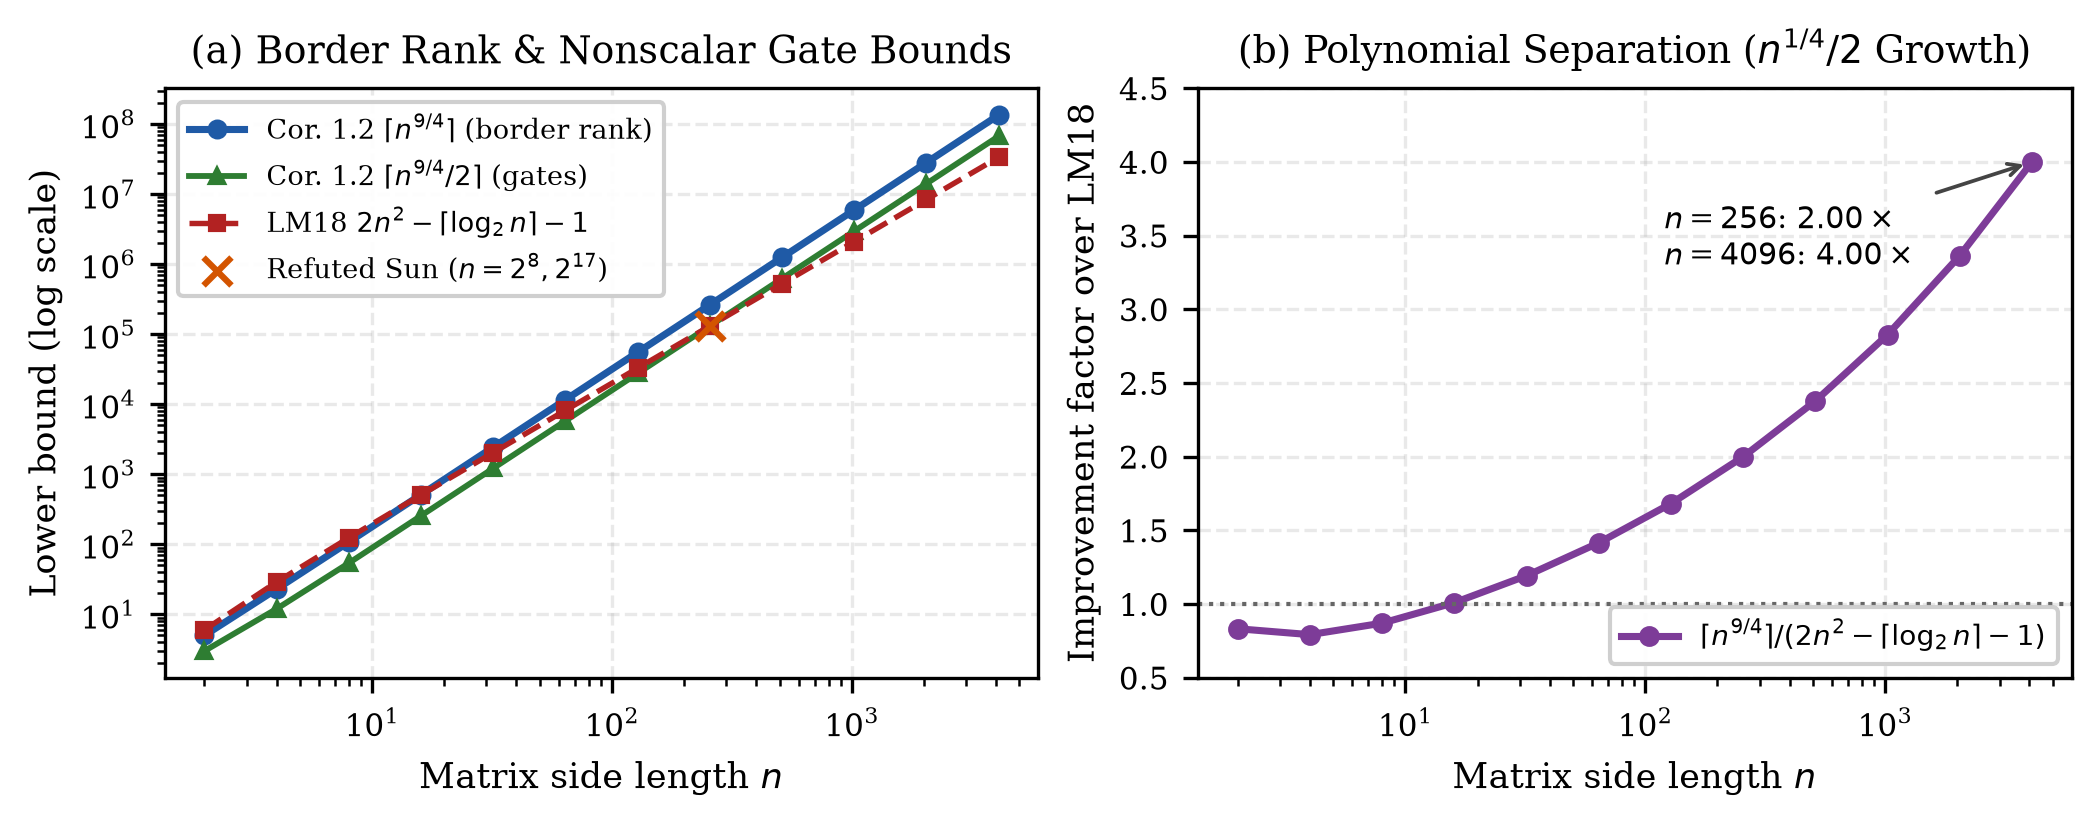
\includegraphics[width=\columnwidth]{figures/fig1_rank_and_gates.png}
\vspace{-1.3em}
\caption{\textbf{(a)}~Exact Corollary~1.2 border-rank ($\lceil n^{9/4}\rceil$) and nonscalar gate ($\lceil n^{9/4}/2\rceil$) lower bounds vs.\ Landsberg--Micha{\l}ek~\cite{landsberg2018lower} ($2n^2-\lceil\log_2 n\rceil-1$), highlighting the refuted Sun $n=2^8, 2^{17}$ point~\cite{sun2026tensor}. \textbf{(b)}~Exact improvement factor over LM18 growing as $n^{1/4}/2$ ($2.00\times$ at $n=256$, $4.00\times$ at $n=4096$).}
\label{fig:rank}
\end{figure}

\begin{figure}[t]
\centering
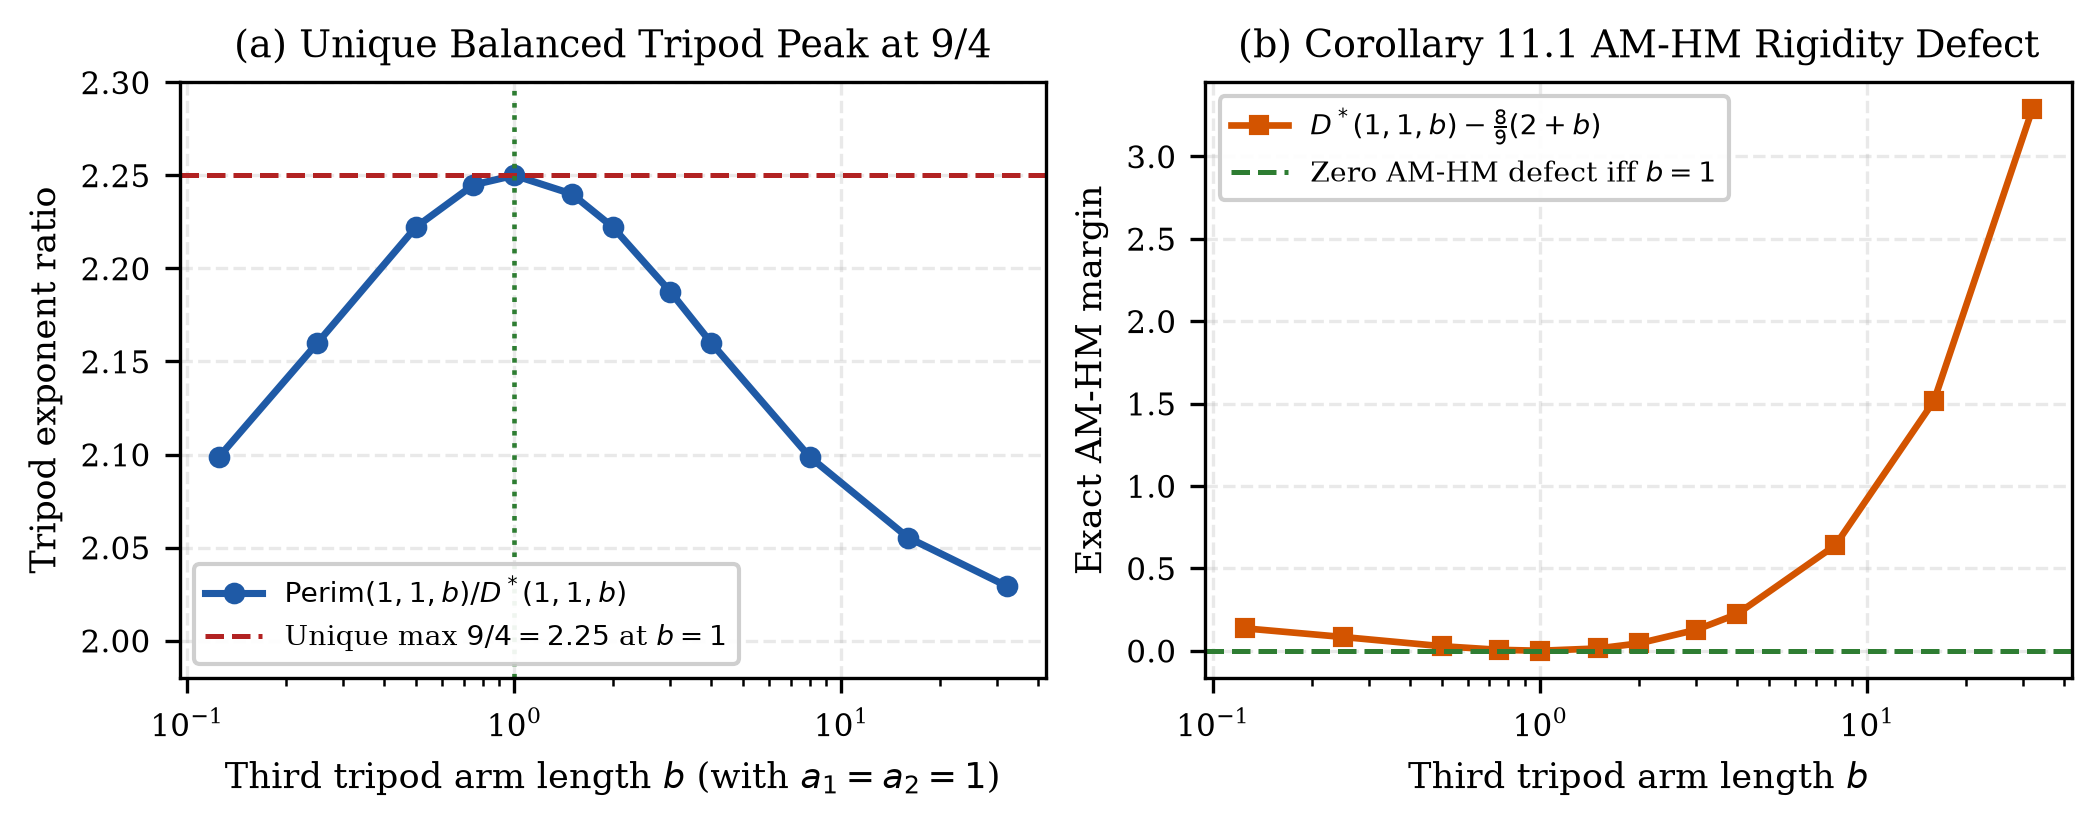
\includegraphics[width=\columnwidth]{figures/fig2_tripod_rigidity.png}
\vspace{-1.3em}
\caption{\textbf{(a)}~Tripod ratio $\mathrm{Perim}(1,1,b)/D^*(1,1,b)$ attaining its unique global maximum $9/4=2.25$ at $b=1$. \textbf{(b)}~Corollary~11.1 AM--HM rigidity defect $D^*(1,1,b)-\frac{8}{9}(2+b)$ vanishing iff $b=1$.}
\label{fig:tripod}
\end{figure}

\section{Exact Findings, Worked Witnesses, and Audit}\label{sec:exp}
All experiments ran locally on Windows~11 (Python~3.12.6, Lean~4.35.0; 7-run means after warm-up).

\paragraph{1. Finite-Size Separation, Tripod Rigidity \& Exhaustive $\mathrm{Tag}(1,1)$ (Figs.~\ref{fig:rank}--\ref{fig:tripod}).}
Exact integer-ceiling sweeps across $n\in\{2,4,\dots,4096\}$ show Corollary~1.2's $\lceil n^{9/4}\rceil$ surpassing Landsberg--Micha{\l}ek's $2n^2-\lceil\log_2 n\rceil-1$ by $2.00\times$ at $n=256$ ($262{,}144$ vs.\ $131{,}063$) and $4.00\times$ at $n=4096$ ($134{,}217{,}728$ vs.\ $33{,}554{,}419$). Figure~\ref{fig:tripod} plots exact rational evaluations of $D^*(1,1,b)$ across $b\in[1/8,32]$: the ratio $\mathrm{Perim}/D^*$ peaks uniquely at $9/4$ for $b=1$ (zero AM--HM defect) and drops to $11/5=2.20$ at $(1,2,3)$ (defect $4/33$) and $20502/10201\approx 2.0098$ at $(1,1,100)$ (defect $726/67$). Exhaustively enumerating all $2^6=64$ inputs to $\mathrm{Tag}(1,1)$ confirms $64/64$ exact agreement (8 accepted, 56 rejected) with Section~4.1's two-$D_w$ signed-sum reduction.

\begin{figure}[t]
\centering
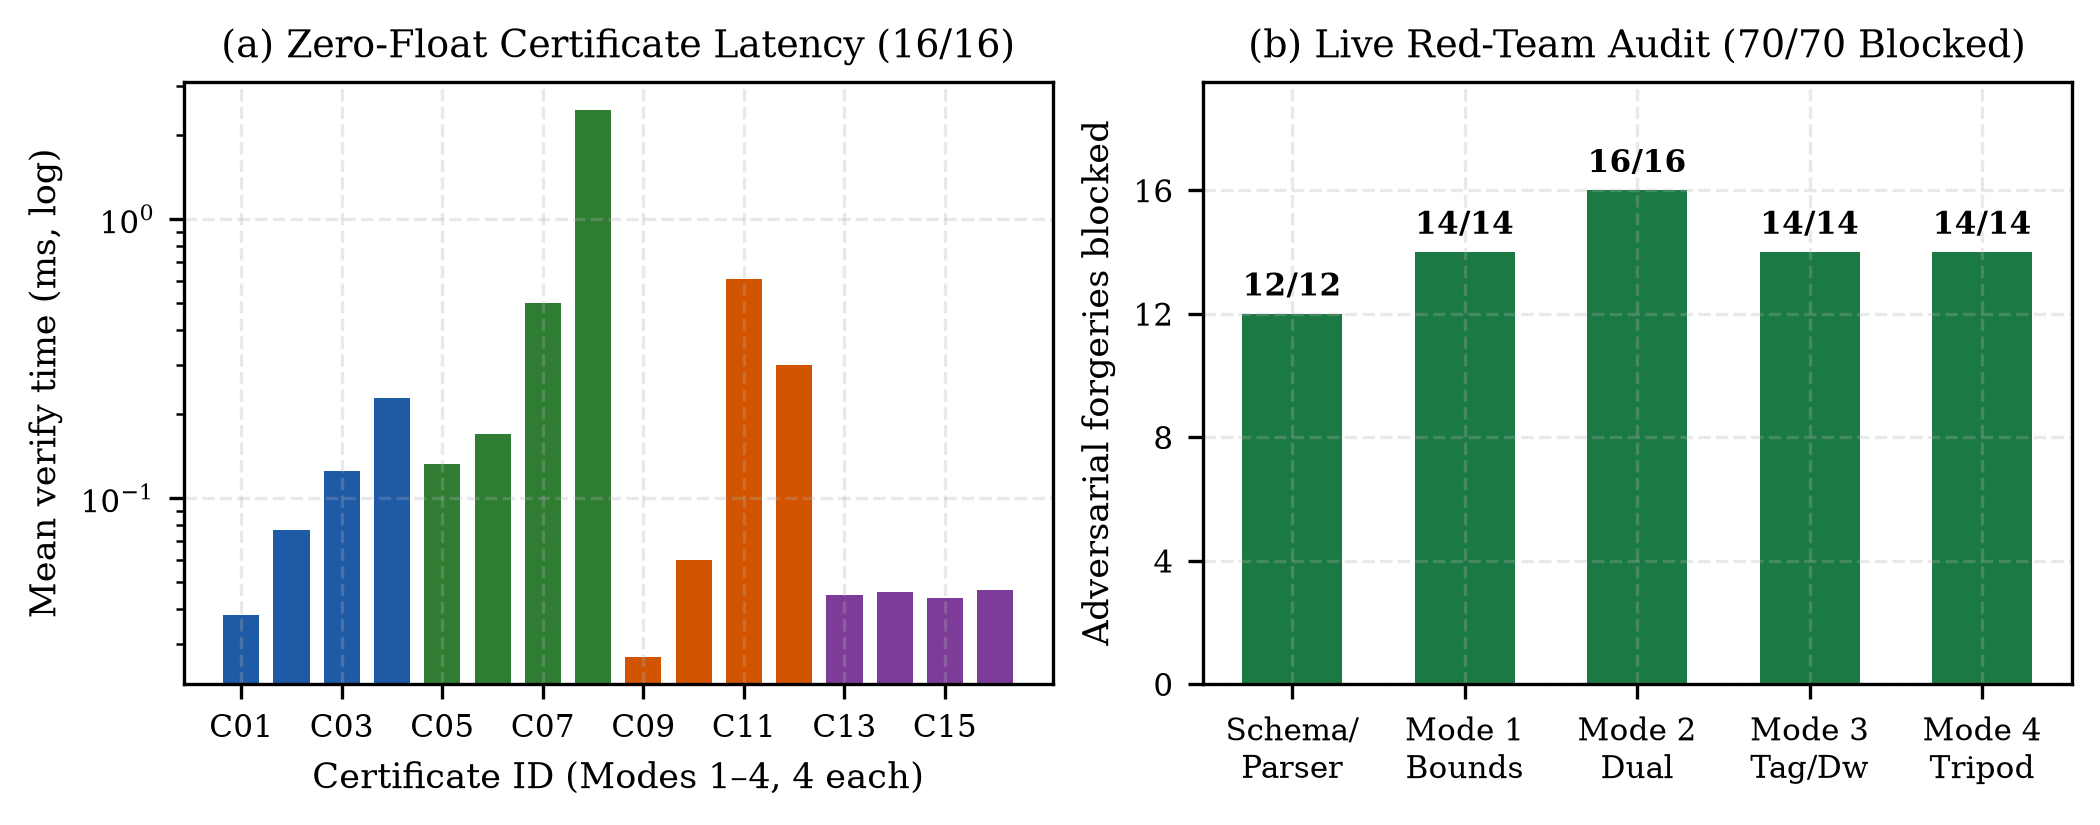
\includegraphics[width=\columnwidth]{figures/fig3_atlas_and_redteam.png}
\vspace{-1.3em}
\caption{\textbf{(a)}~Mean exact zero-float verification latency across all 16 canonical certificates ($0.027$--$2.466\,\mathrm{ms}$, log scale). \textbf{(b)}~Live adversarial red-team audit rejecting 70/70 forgeries across five attack classes with exact error-branch assertions.}
\label{fig:atlas}
\end{figure}

\paragraph{2. Hand-Verifiable Worked Exact Witnesses (One per Mode).}
\begin{itemize}[leftmargin=1.2em,itemsep=1pt,topsep=2pt]
  \item \textbf{Mode~1 (\texttt{C02}, $n=256=2^8$, rect $(16,4,16)$, tight $T_6$):} $256^9 = 2^{72} = (2^{18})^4$, certifying border rank $\ge 262{,}144 > 2^{17}=131{,}072$ (refuting Sun~\cite{sun2026tensor}) and $\ge 131{,}072$ nonscalar gates; for $T_{16,4,16}$, $(1024)^{3/4}\approx 181.0 < \max(64,64,256)=256$; for $T_6$ with $B=7$, all $6^3=216$ triples satisfy $(i-7j)+(7j-49k)+(49k-i)=0$ with $36$ distinct weights per factor.
  \item \textbf{Mode~2 (\texttt{C06}, $2{\times}2$ Strassen + division over $\FF_{257}[X,Y][u,v]/(u^2,v^2)$):} Routing $M_1$ through $(M_1 d)/d$ with regular nonconstant $d=a_{00}+b_{11}+1$ uses 30 gates ($q=9$ symbolically nonscalar: 8 \texttt{mul} + 1 \texttt{div}, Lemma~2.4 rank bound $2q=18$) and symbolically matches $(A_0+uX)(B_0+vY)$ across all $1+8+16=25$ coordinates per output entry modulo 257.
  \item \textbf{Mode~3 (\texttt{C10}, $\mathrm{Tag}(2,2)$, $N=4$):} On valid permutation $\pi=[2,0,3,1]$ with $x=[1,3,2,0], y=[3,0,1,2]$ ($x_i=y_{\pi(i)}$), $D_w^{(1)}=1$ and the $2^4=16$-term signed sum yields $+1$; mutating $x_3\to 1$ collapses the signed sum to $0$, and colliding $\pi_2\to 2$ gives $D_w^{(1)}=0$.
  \item \textbf{Mode~4 (\texttt{C13} \& \texttt{C14}):} On $(1,1,1)$, $D^*=3-\frac{1}{3}=\frac{8}{3}$, perimeter $=6$, ratio $=6/(8/3)=9/4$, AM--HM margin $=0$, and $D^*(1,1,5)=7-\frac{5}{11}=\frac{72}{11}=5+\frac{3}{2}+\frac{1}{22}$. On scale-1 maximal $(\frac{3}{8},\frac{3}{8},\frac{3}{8})$ (Cor.~11.1), $D^*=1$, all three wire lengths equal $\frac{3}{4}$, and perimeter $=9/4$.
\end{itemize}

\begin{table}[t]
\centering
\caption{Canonical 16-certificate \texttt{OMEGA94-\allowbreak LB-\allowbreak CERT-1.0} atlas (\texttt{exp1\_\allowbreak certificate\_\allowbreak atlas.json}; all 16 verified).}
\label{tab:atlas}
\scriptsize
\setlength{\tabcolsep}{1.9pt}
\resizebox{\columnwidth}{!}{%
\begin{tabular}{@{}c l c l r@{}}
\toprule
ID & Certificate Name & M & Exact Certified Witness Summary & ms \\
\midrule
C01 & \texttt{m1\_bounds\_n16\_rect4x4x4} & M1 & $n{=}16$: $\underline{R}\ge 512$, gates $\ge 256$, $T_{4,4,4}\ge 23$ & 0.038 \\
C02 & \texttt{m1\_bounds\_n256\_sun\_refute} & M1 & $n{=}256$: $\underline{R}\ge 2^{18}>2^{17}$, gates $\ge 131072$ & 0.077 \\
C03 & \texttt{m1\_bounds\_n1024\_rect64x16x64} & M1 & $n{=}1024$: $\underline{R}\ge 5931642$, $T_8$ ($512$ triples) & 0.125 \\
C04 & \texttt{m1\_bounds\_n4096\_rect256x64x256} & M1 & $n{=}4096$: $\underline{R}\ge 2^{27}$, $T_{10}$ ($1000$ triples) & 0.229 \\
C05 & \texttt{m2\_dual\_strassen\_2x2\_f101} & M2 & $\FF_{101}$, $2{\times}2$ Strassen: $q{=}7$, $2q{=}14$ & 0.132 \\
C06 & \texttt{m2\_dual\_strassen\_div\_2x2\_f257} & M2 & $\FF_{257}$, $2{\times}2$ Strassen+div: $q{=}9$, $2q{=}18$ & 0.169 \\
C07 & \texttt{m2\_dual\_schoolbook\_div\_3x3\_f509} & M2 & $\FF_{509}$, $3{\times}3$ +div: $q{=}29$, $2q{=}58$ & 0.499 \\
C08 & \texttt{m2\_dual\_schoolbook\_4x4\_f1009} & M2 & $\FF_{1009}$, $4{\times}4$ symbolic: $q{=}64$, $2q{=}128$ & 2.466 \\
C09 & \texttt{m3\_tag\_h1\_exhaustive\_4cases} & M3 & $\mathrm{Tag}(1,1)$ ($N{=}2$): 4 instances (2 acc.) & 0.027 \\
C10 & \texttt{m3\_tag\_h2\_valid\_and\_collisions} & M3 & $\mathrm{Tag}(2,2)$ ($N{=}4$): 4 instances (16 masks) & 0.060 \\
C11 & \texttt{m3\_tag\_h3\_cyclic\_perm\_n8} & M3 & $\mathrm{Tag}(3,3)$ ($N{=}8$): cyclic (256 masks) & 0.610 \\
C12 & \texttt{m3\_tag\_h3\_involution\_n8} & M3 & $\mathrm{Tag}(3,3)$ ($N{=}8$): invol.\ (256 masks) & 0.301 \\
C13 & \texttt{m4\_tripod\_balanced\_unit\_1\_1\_1} & M4 & $(1,1,1)$: $D^*{=}8/3$, ratio $9/4$, margin $0$ & 0.045 \\
C14 & \texttt{m4\_tripod\_maximal\_scale1\_3\_8} & M4 & $(\frac{3}{8},\frac{3}{8},\frac{3}{8})$: $D^*{=}1$, wires $\frac{3}{4}$, $9/4$ & 0.046 \\
C15 & \texttt{m4\_tripod\_asymmetric\_1\_2\_3} & M4 & $(1,2,3)$: $D^*{=}60/11$, ratio $11/5$, marg.\ $4/33$ & 0.044 \\
C16 & \texttt{m4\_tripod\_stretched\_1\_1\_100} & M4 & $(1,1,100)$: ratio $20502/10201$, $b{=}100$ & 0.047 \\
\bottomrule
\end{tabular}}
\end{table}

\paragraph{3. 16-Certificate Atlas \& 76-Test Red-Team Audit (Table~\ref{tab:atlas}, Fig.~\ref{fig:atlas}).}
Table~\ref{tab:atlas} lists all 16 canonical certificates verified in $0.027$--$2.466\,\mathrm{ms}$. \texttt{tests/test\_\allowbreak suite.py} runs 76 pytest checks: 1 full 16-certificate replay, 3 raw-JSON parser guards (float, \texttt{NaN}, duplicate keys), 2 exact regressions (exhaustive 64-input $\mathrm{Tag}(1,1)$ agreement and balanced tripod peak / Sun $n=256$ refutation), and 70 parametrized live adversarial forgeries (12 schema/parser, 14 Mode~1, 16 Mode~2 including a $q{=}1$ single-direction cheat and noncanonical field/constant entries, 14 Mode~3, and 14 Mode~4 including a forged zero-column-sum star matrix), each asserting an exact regex on its intended \texttt{CertificateError} branch. \texttt{scripts/verify\_\allowbreak all.py} enforces all 5 gates including strict axiom whitelisting and a 41-file SHA-256 manifest.

\section{Conclusion}\label{sec:conc}
We built an independent, explicitly scoped, zero-floating-point verification companion for the discrete algebraic, symbolic dual-number bilinearization, tight-tensor, tagged-permutation, harmonic-star, and tripod AM--HM rigidity mechanisms of OpenAI's $\omega_F=9/4$ lower-bound preprint~\cite{openai2026omega94}, pairing 18 constructive Lean~4.35.0 sub-lemmas (zero \texttt{sorry}, zero \texttt{Classical.choice}) with the pure-\texttt{int}/\texttt{Fraction} 4-mode auditor \texttt{OMEGA94-\allowbreak LB-\allowbreak CERT-1.0}, 16 canonical exact finite witnesses, and 70/70 live adversarial forgery rejections.

{\footnotesize
\bibliographystyle{plain}
\bibliography{references}}
\end{document}
